% This file was created by matplotlib2tikz v0.6.18.
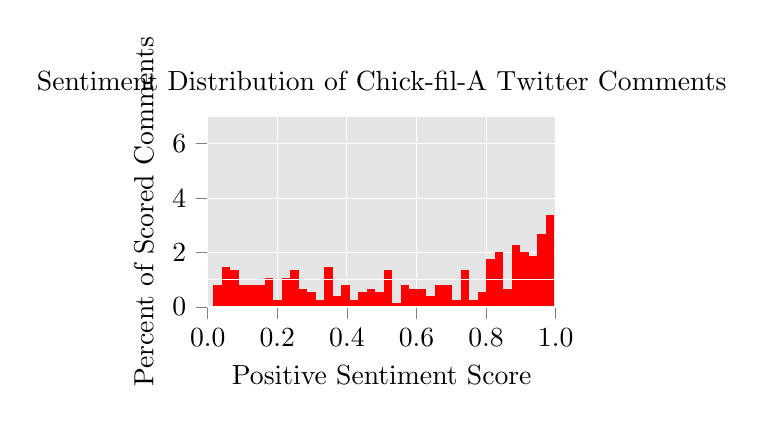
\begin{tikzpicture}

\begin{axis}[
axis background/.style={fill=white!89.80392156862746!black},
axis line style={white},
height=4cm,
tick align=outside,
tick pos=left,
title={Sentiment Distribution of Chick-fil-A Twitter Comments},
width=6cm,
x grid style={white},
xlabel={Positive Sentiment Score},
xmajorgrids,
xmin=0, xmax=1,
xtick={0,0.2,0.4,0.6,0.8,1},
xticklabels={0.0,0.2,0.4,0.6,0.8,1.0},
y grid style={white},
ylabel={Percent of Scored Comments},
ymajorgrids,
ymin=0, ymax=7
]
\draw[fill=red,draw opacity=0] (axis cs:0.0161207467317581,0) rectangle (axis cs:0.0406186208128929,0.808314167459386);
\draw[fill=red,draw opacity=0] (axis cs:0.0406186208128929,0) rectangle (axis cs:0.0651164948940277,1.48190941968278);
\draw[fill=red,draw opacity=0] (axis cs:0.0651164948940277,0) rectangle (axis cs:0.0896143689751625,1.3471903815298);
\draw[fill=red,draw opacity=0] (axis cs:0.0896143764257431,0) rectangle (axis cs:0.114112250506878,0.80831422891788);
\draw[fill=red,draw opacity=0] (axis cs:0.114112250506878,0) rectangle (axis cs:0.138610124588013,0.808313983083958);
\draw[fill=red,draw opacity=0] (axis cs:0.138610124588013,0) rectangle (axis cs:0.163107991218567,0.808314474751953);
\draw[fill=red,draw opacity=0] (axis cs:0.163107991218567,0) rectangle (axis cs:0.187605872750282,1.07775197744528);
\draw[fill=red,draw opacity=0] (axis cs:0.187605887651443,0) rectangle (axis cs:0.212103769183159,0.269437994361319);
\draw[fill=red,draw opacity=0] (axis cs:0.212103754281998,0) rectangle (axis cs:0.236601620912552,1.0777526330026);
\draw[fill=red,draw opacity=0] (axis cs:0.236601620912552,0) rectangle (axis cs:0.261099487543106,1.34719079125325);
\draw[fill=red,draw opacity=0] (axis cs:0.261099517345428,0) rectangle (axis cs:0.285597413778305,0.673594576180468);
\draw[fill=red,draw opacity=0] (axis cs:0.285597383975983,0) rectangle (axis cs:0.310095250606537,0.538876316501302);
\draw[fill=red,draw opacity=0] (axis cs:0.310095250606537,0) rectangle (axis cs:0.334593117237091,0.269438158250651);
\draw[fill=red,draw opacity=0] (axis cs:0.334593117237091,0) rectangle (axis cs:0.359090983867645,1.48190987037858);
\draw[fill=red,draw opacity=0] (axis cs:0.359090983867645,0) rectangle (axis cs:0.383588880300522,0.404156745708281);
\draw[fill=red,draw opacity=0] (axis cs:0.383588880300522,0) rectangle (axis cs:0.408086746931076,0.808314474751953);
\draw[fill=red,draw opacity=0] (axis cs:0.408086746931076,0) rectangle (axis cs:0.43258461356163,0.269438158250651);
\draw[fill=red,draw opacity=0] (axis cs:0.432584643363953,0) rectangle (axis cs:0.457082539796829,0.538875660944374);
\draw[fill=red,draw opacity=0] (axis cs:0.457082509994507,0) rectangle (axis cs:0.481580376625061,0.673595395626627);
\draw[fill=red,draw opacity=0] (axis cs:0.481580376625061,0) rectangle (axis cs:0.506078243255615,0.538876316501302);
\draw[fill=red,draw opacity=0] (axis cs:0.506078243255615,0) rectangle (axis cs:0.530576109886169,1.34719079125325);
\draw[fill=red,draw opacity=0] (axis cs:0.530576109886169,0) rectangle (axis cs:0.555073976516724,0.134719079125325);
\draw[fill=red,draw opacity=0] (axis cs:0.555073976516724,0) rectangle (axis cs:0.579571902751923,0.808312508083563);
\draw[fill=red,draw opacity=0] (axis cs:0.579571902751923,0) rectangle (axis cs:0.604069769382477,0.673595395626627);
\draw[fill=red,draw opacity=0] (axis cs:0.604069769382477,0) rectangle (axis cs:0.628567636013031,0.673595395626627);
\draw[fill=red,draw opacity=0] (axis cs:0.628567636013031,0) rectangle (axis cs:0.653065502643585,0.404157237375976);
\draw[fill=red,draw opacity=0] (axis cs:0.653065502643585,0) rectangle (axis cs:0.677563369274139,0.808314474751953);
\draw[fill=red,draw opacity=0] (axis cs:0.677563369274139,0) rectangle (axis cs:0.702061235904694,0.808314474751953);
\draw[fill=red,draw opacity=0] (axis cs:0.702061235904694,0) rectangle (axis cs:0.726559102535248,0.269438158250651);
\draw[fill=red,draw opacity=0] (axis cs:0.726559042930603,0) rectangle (axis cs:0.751056969165802,1.34718751347261);
\draw[fill=red,draw opacity=0] (axis cs:0.751057028770447,0) rectangle (axis cs:0.775554895401001,0.269438158250651);
\draw[fill=red,draw opacity=0] (axis cs:0.775554895401001,0) rectangle (axis cs:0.800052762031555,0.538876316501302);
\draw[fill=red,draw opacity=0] (axis cs:0.800052762031555,0) rectangle (axis cs:0.824550628662109,1.75134802862923);
\draw[fill=red,draw opacity=0] (axis cs:0.824550628662109,0) rectangle (axis cs:0.849048495292664,2.02078618687988);
\draw[fill=red,draw opacity=0] (axis cs:0.849048495292664,0) rectangle (axis cs:0.873546361923218,0.673595395626627);
\draw[fill=red,draw opacity=0] (axis cs:0.873546361923218,0) rectangle (axis cs:0.898044228553772,2.29022434513053);
\draw[fill=red,draw opacity=0] (axis cs:0.898044228553772,0) rectangle (axis cs:0.922542154788971,2.02078127020891);
\draw[fill=red,draw opacity=0] (axis cs:0.922542154788971,0) rectangle (axis cs:0.947040021419525,1.88606710775456);
\draw[fill=red,draw opacity=0] (axis cs:0.947040021419525,0) rectangle (axis cs:0.971537888050079,2.69438158250651);
\draw[fill=red,draw opacity=0] (axis cs:0.971537888050079,0) rectangle (axis cs:0.996035754680634,3.36797697813314);
\path [draw=white, fill opacity=0] (axis cs:0,0)
--(axis cs:0,7);

\path [draw=white, fill opacity=0] (axis cs:1,0)
--(axis cs:1,7);

\path [draw=white, fill opacity=0] (axis cs:0,0)
--(axis cs:1,0);

\path [draw=white, fill opacity=0] (axis cs:0,1)
--(axis cs:1,1);

\end{axis}

\end{tikzpicture}